\begin{usecase}{Connect Calendar}
    \ucbasicinfo{Medium}{Regular}
    \ucshortdescription{This UC allows the user to access their iOS device calendars through EventKit and configure CalDAV accounts.}
    \uctrigger{This UC is triggered when the user first launches the app or manually initiates calendar access.}
    \ucactors{User}{EventKit}
    \ucpreconditions{User must be logged in}
    \ucrelationships{N/A}{N/A}{N/A}
    \ucinputsoutputs{
        \begin{itemize}
            \item \textbf{Calendar Access Permission} (Source: User)
            \item \textbf{CalDAV Account Credentials} (Source: Backend)
        \end{itemize}
    }{
        \begin{itemize}
            \item \textbf{Local Calendar Access Status} (Destination: System)
            \item \textbf{Calendar Events} (Destination: App)
        \end{itemize}
    }
    \ucmainflow{
        \begin{enumerate}
            \item The system requests calendar access permission from the user.
                  \ucinfo{The app requests EventKit authorization to access device calendars.}
            \item The system retrieves CalDAV account credentials from the backend.
                  \ucinfo{The app fetches encrypted credentials for our CalDAV server.}
            \item The system configures CalDAV accounts through iOS's native calendar system.
                  \ucinfo{EventKit handles direct communication with all CalDAV servers (both ours and external ones).}
            \item The system fetches calendar events using EventKit.
                  \ucinfo{Events are fetched from all configured calendar accounts through iOS's native calendar system.}
            \item The system sets up local notifications for calendar events.
                  \ucinfo{Notifications are scheduled locally based on event reminders.}
        \end{enumerate}
    }
    \ucalternateflows{
        \begin{enumerate}
            \item If calendar access is denied, the user can grant permission through device settings.
            \item If account configuration fails, the user can retry the connection through iOS settings.
        \end{enumerate}
    }
    \ucexceptions{
        \begin{itemize}
            \item Calendar access permission denied
            \item Network issue retrieving account credentials
            \item iOS calendar account configuration failure
        \end{itemize}
    }
    \ucconclusion{The UC ends when the user has access to their device calendars and CalDAV accounts are configured in iOS.}
    \ucpostconditions{The app can read calendar events through EventKit from all configured calendar sources.}
    \ucspecialrequirements{The system must rely on iOS's native calendar system for all CalDAV communication.}
\end{usecase}

\begin{figure}[!h]
    \centering
    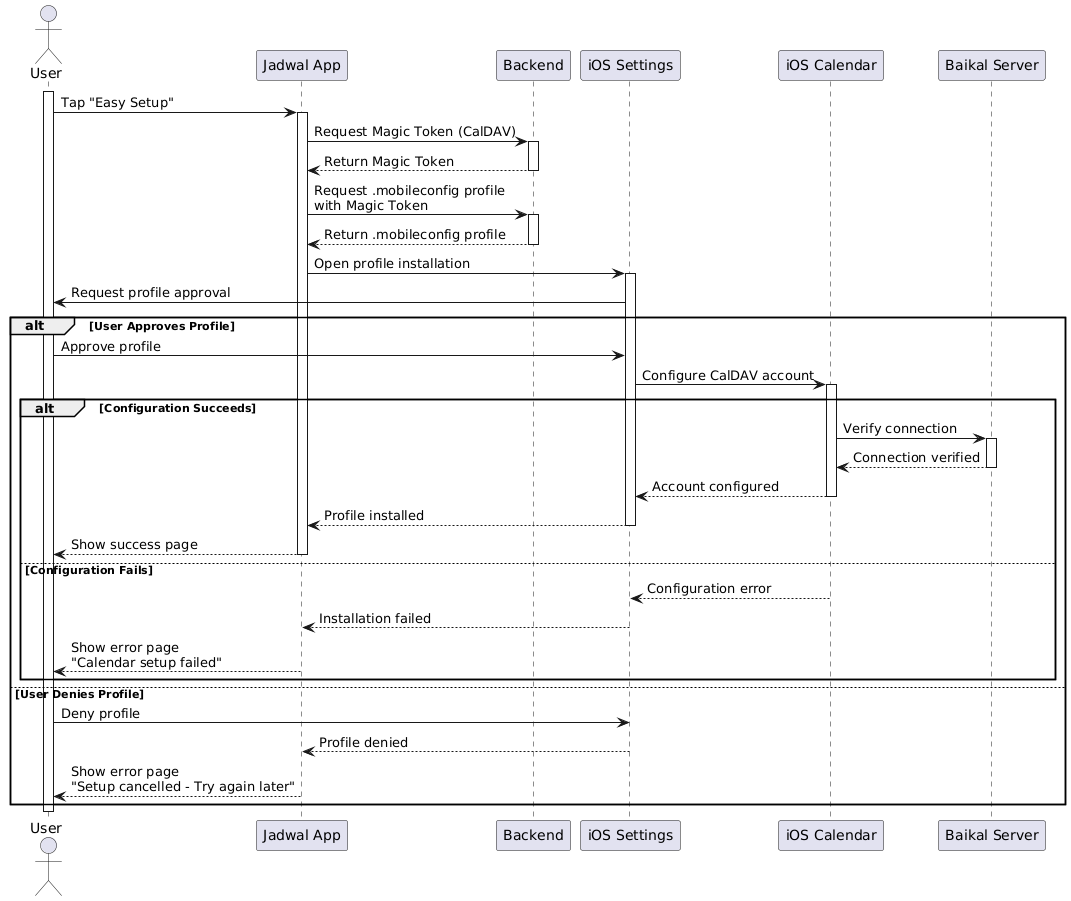
\includegraphics[width=\textwidth]{images/docs/diagrams/sequence-diagrams/all-sequence-diagrams/Connect Calendar.png}
    \caption{Connect Calendar Sequence Diagram}
    \label{fig:seq/connect-calendar}
\end{figure}

The ``Connect Calendar Sequence Diagram'', shown in \textbf{Figure~\ref{fig:seq/connect-calendar}}, illustrates the calendar integration process:

\begin{enumerate}
    \item \textbf{Local Calendar Access:} The iOS app uses EventKit framework to request and manage access to the device's calendars. This provides direct access to the user's existing calendar data.

    \item \textbf{Account Configuration:} The app retrieves encrypted CalDAV account credentials from the backend and uses iOS's native calendar system to configure the accounts. EventKit and iOS handle all direct communication with CalDAV servers, both our own and external ones.
\end{enumerate}

The Backend's role is strictly limited to securely storing and providing encrypted CalDAV account credentials. All calendar data synchronization, CalDAV communication, and event management happens through iOS's native calendar system using EventKit. This approach leverages iOS's built-in CalDAV client capabilities, ensuring reliable calendar synchronization while maintaining security of sensitive credentials.